\documentclass[11pt]{article}

\usepackage[T1]{fontenc}
\usepackage[utf8]{inputenc}
\usepackage{lmodern}
\usepackage{microtype}
\usepackage[margin=1in]{geometry}
\usepackage{amsmath,amssymb,bm}
\usepackage{booktabs}
\usepackage{enumitem}
\usepackage[numbers,sort&compress]{natbib}
\usepackage{graphicx}
\usepackage{xcolor}
\usepackage{xurl}
\usepackage{hyperref}
\usepackage[nameinlink,noabbrev]{cleveref}
\usepackage{caption}
\usepackage[section]{placeins}
\captionsetup{font=small,labelfont=bf}
\graphicspath{{../../plots/writeup/}{../../plots/}{../../plots/candidates/}}

\hypersetup{colorlinks=true,linkcolor=blue,citecolor=blue,urlcolor=blue,
  pdftitle={Binary RR Lyrae in the LMC: what the O-C measures and how the pipeline works}}

\newcommand{\Msun}{\ensuremath{M_\odot}}
\newcommand{\kms}{\ensuremath{\mathrm{km\,s^{-1}}}}
\newcommand{\OC}{\ensuremath{O{-}C}}
\newcommand{\Pdot}{\ensuremath{\dot P}}

\title{\bf Binary RR Lyrae in the LMC from the light-travel-time effect\\
\large What we measure (the \OC\ diagram), mock illustrations, and the pipeline}
\author{Project \texttt{rrl\_lmc\_binary} --- working note}
\date{30 September 2026 (code: \url{https://github.com/vasilybelokurov/rrl_lmc_binary})}

\begin{document}
\maketitle

\begin{abstract}
An RR Lyrae star pulsates with a period of about half a day and a very stable, sharply shaped light curve, so it
can be used as a clock. If it orbits a companion, its distance from us changes periodically and the pulsation
signal arrives earlier or later by the light-travel time across the orbit --- minutes to tens of minutes for
companions of $0.1$--$1\,\Msun$ on 3--30-yr orbits. We measure this delay once per observing season for
17{,}492 LMC RRab stars with OGLE-II/III/IV photometry (1997--2016) and, for 6{,}614 of them, MACHO photometry
(1992--1999). The resulting time series of delays is the \OC\ diagram. This note explains the measurement in
words and in equations, illustrates it with mock data, and documents the pipeline, its tests and its known
limitations. Results are summarized only briefly (\cref{sec:status}): they are being recomputed after a fix
to the orbital-period search (\cref{sec:nyquist}).
\end{abstract}

\tableofcontents

%==============================================================================
\section{What we measure, in simple words}\label{sec:words}

\begin{enumerate}[leftmargin=*]
\item \textbf{The clock.} An RRab star brightens steeply (within about an hour) and fades slowly, repeating every
$P\approx0.5$--$0.7$\,d. The shape repeats almost exactly, so the times of the steep rise are sharp time markers.
\item \textbf{The prediction.} From the catalogue period and one reference epoch we predict when the rise should
happen in any later year: the ``calculated'' time $C$.
\item \textbf{The observation.} In each observing season we find the time shift that best lines up the observed light
curve with the star's own template: the ``observed'' time $O$. The difference $O-C$ is the \emph{delay} of that season.
\item \textbf{What changes the delay.} (i) A slightly wrong catalogue period makes $O-C$ grow linearly with time.
(ii) A slow, steady change of the period (stellar evolution) bends $O-C$ into a parabola.
(iii) An orbiting companion moves the RR Lyrae towards and away from us; the light has a little further or a little
less distance to travel, so $O-C$ oscillates with the orbital period (\cref{fig:orbit}). This is the
light-travel-time effect (LTTE).
(iv) The star itself can change its period irregularly (jumps, wander, Blazhko modulation); this also moves
$O-C$ and is the main confusion.
\item \textbf{Why it works at the LMC.} The delay depends only on the size of the orbit, not on the distance to the star.
A $0.6\,\Msun$ companion on a 3000-d orbit gives $\pm17.5$\,min everywhere in the Universe. The price of the LMC
distance is photometric noise: our stars are at $I\approx19$, so one season's delay is measured to about 4\,min (median).
\item \textbf{What we look for.} A delay that oscillates smoothly and repeats, with the same amplitude in every band and
survey, on top of an ordinary smooth period change; and, statistically, how many such stars there are.
\end{enumerate}

%==============================================================================
\section{What we measure, in equations}\label{sec:eqs}

\subsection{Light curve, ephemeris and delay}
Let $T(\phi)$ be the star's mean light curve (template) as a function of pulsation phase $\phi\in[0,1)$, written as a
Fourier series of order $K$ (we use $K=8$),
\begin{equation}
T(\phi)=\sum_{k=1}^{K}\left[a_k\cos(2\pi k\phi)+b_k\sin(2\pi k\phi)\right].
\end{equation}
With a reference period $P$ and epoch $T_0$ (the OGLE-IV catalogue values), the observed magnitude is modelled as
\begin{equation}\label{eq:lc}
m(t)=z_s+\delta m_j+\alpha_j\,T\!\left(\frac{t-\tau_j-T_0}{P}\right)+\varepsilon ,
\end{equation}
where $s$ labels the survey segment (OGLE-II, -III, -IV, MACHO; separate zero points $z_s$), $j$ the observing season,
$\tau_j$ the season's delay, $\delta m_j$ a mean-magnitude offset and $\alpha_j$ an amplitude factor (both nuisance
parameters; $\alpha_j$ is also a Blazhko diagnostic), and $\varepsilon$ the photometric noise. A single $\tau_j$ shifts all
harmonics together: this is what a change in light-travel time does. The set $\{\tau_j\}$ versus time is the
\OC\ diagram; $\tau>0$ means the pulsation arrives late.

\subsection{Ordinary period change: the quadratic}
If the period changes slowly and steadily, $P(t)=P_0+\Pdot\,t$, the $n$-th maximum occurs at
$T_n=T_0'+nP_0+\tfrac12\Pdot P_0 n^2$, and with $n\simeq t/P_0$
\begin{equation}\label{eq:quad}
\tau(t)=c_0+c_1\,t+c_2\,t^2,\qquad c_1=\frac{P_0-P}{P},\qquad c_2=\frac{\Pdot}{2P}.
\end{equation}
$c_0$ is an uninteresting constant (epoch and template-phase convention), $c_1$ a period error, $c_2$ the rate of
period change. For an evolutionary $\Pdot=0.1$\,d\,Myr$^{-1}$ ($2.7\times10^{-10}$\,d\,d$^{-1}$) and $P=0.55$\,d,
$c_2=2.5\times10^{-10}$\,d$^{-1}$, i.e.\ $\tau\approx2.5\times10^{-10}\times(4000)^2$\,d $=0.004$\,d $\approx350$\,s
at 4000\,d from the reference epoch: comparable to the orbital signals, so the quadratic is always part of the model.

\subsection{Light-travel-time effect}
If the RR Lyrae (mass $M_1$) orbits a companion ($M_2$), the delay is its line-of-sight position divided by $c$
\citep{Irwin1952}:
\begin{equation}\label{eq:ltte}
\tau_{\rm LTTE}(t)=\frac{a_1\sin i}{c}\;\frac{1-e^2}{1+e\cos\nu(t)}\,\sin\!\big(\nu(t)+\omega\big),
\end{equation}
with true anomaly $\nu$ from Kepler's equation, eccentricity $e$, argument of periastron $\omega$, and
\begin{equation}
a_1=\left[\frac{G(M_1+M_2)P_{\rm orb}^2}{4\pi^2}\right]^{1/3}\frac{M_2}{M_1+M_2}.
\end{equation}
From the fitted $P_{\rm orb}$ and semi-amplitude $A\equiv a_1\sin i/c$ one obtains the mass function
\begin{equation}\label{eq:fm}
f(M_2)=\frac{4\pi^2(cA)^3}{G P_{\rm orb}^2}=\frac{(M_2\sin i)^3}{(M_1+M_2)^2},
\end{equation}
and the primary's radial-velocity semi-amplitude $K_1=2\pi c A/[P_{\rm orb}\sqrt{1-e^2}]$.
The full \OC\ model is $\tau(t)=c_0+c_1t+c_2t^2+\tau_{\rm LTTE}(t)$.

\begin{table}[h]
\centering
\caption{LTTE semi-amplitude $A=a_1/c$ for $M_1=0.65\,\Msun$, circular, edge-on (\texttt{rrlbin.ltte.a1sini\_over\_c}).}
\label{tab:amp}
\begin{tabular}{rccc}
\toprule
$P_{\rm orb}$ [d] & $M_2=0.6\,\Msun$ & $0.2\,\Msun$ & $0.07\,\Msun$\\
\midrule
1000 & 505\,s & 218\,s & 85\,s\\
3000 & 1050\,s (17.5 min) & 453\,s & 177\,s\\
\bottomrule
\end{tabular}
\end{table}

\subsection{Measuring one season's delay}
For fixed template $(a_k,b_k,z_s)$, each season's $(\tau_j,\delta m_j,\alpha_j)$ is fitted by weighted least squares
(Gauss--Newton after a coarse search over one full cycle). Its Fisher (Cram\'er--Rao) error is
\begin{equation}\label{eq:fisher}
\sigma_{\tau_j}^{-2}\simeq\sum_{i\in j}\frac{1}{\sigma_i^2}\left(\frac{\partial m}{\partial t}\right)_i^2
=\sum_{i\in j}\frac{\alpha_j^2\,T'(\phi_i)^2}{P^2\sigma_i^2},
\end{equation}
scaled by $\sqrt{\max(\chi^2_\nu,1)}$. The steep rising branch dominates the sum. Template and delays are iterated to
convergence. Because a constant delay is degenerate with the template phase, we fix the gauge so that the
template's fundamental harmonic has phase zero.

\subsection{Detection statistic $D$}
On the season delays $\{t_j,\tau_j,\sigma_j\}$ we compare two Gaussian models with variance $\sigma_j^2+s^2$
(extra jitter $s$ fitted in each):
$H_0$: \cref{eq:quad} (+ a free MACHO offset); $H_1$: $H_0$ + $A_s\sin(2\pi t/P_{\rm orb})+A_c\cos(2\pi t/P_{\rm orb})$.
\begin{equation}\label{eq:D}
D=2\max_{P_{\rm orb}}\left[\ln\mathcal L_1(P_{\rm orb})-\ln\mathcal L_0\right].
\end{equation}
At fixed $P_{\rm orb}$ and for white noise $D\sim\chi^2_2$; for $N$ seasons of error $\sigma$ and amplitude $A$,
$D\approx NA^2/(2\sigma^2)$. $D$ tests an orbit against a \emph{smooth} period change plus white noise; it does
not by itself reject irregular intrinsic period changes (\cref{sec:nuis}).

%==============================================================================
\section{Mock-data illustrations}\label{sec:mocks}
All figures in this section are synthetic (\texttt{scripts/plot\_writeup\_mocks.py}); the template is a typical
OGLE $I$-band RRab template (first-harmonic amplitude 0.155\,mag), and the orbit has $M_1=0.65$, $M_2=0.6\,\Msun$,
$P_{\rm orb}=3000$\,d, $e=0.3$, $i=90^\circ$.

\begin{figure}[h]
\centering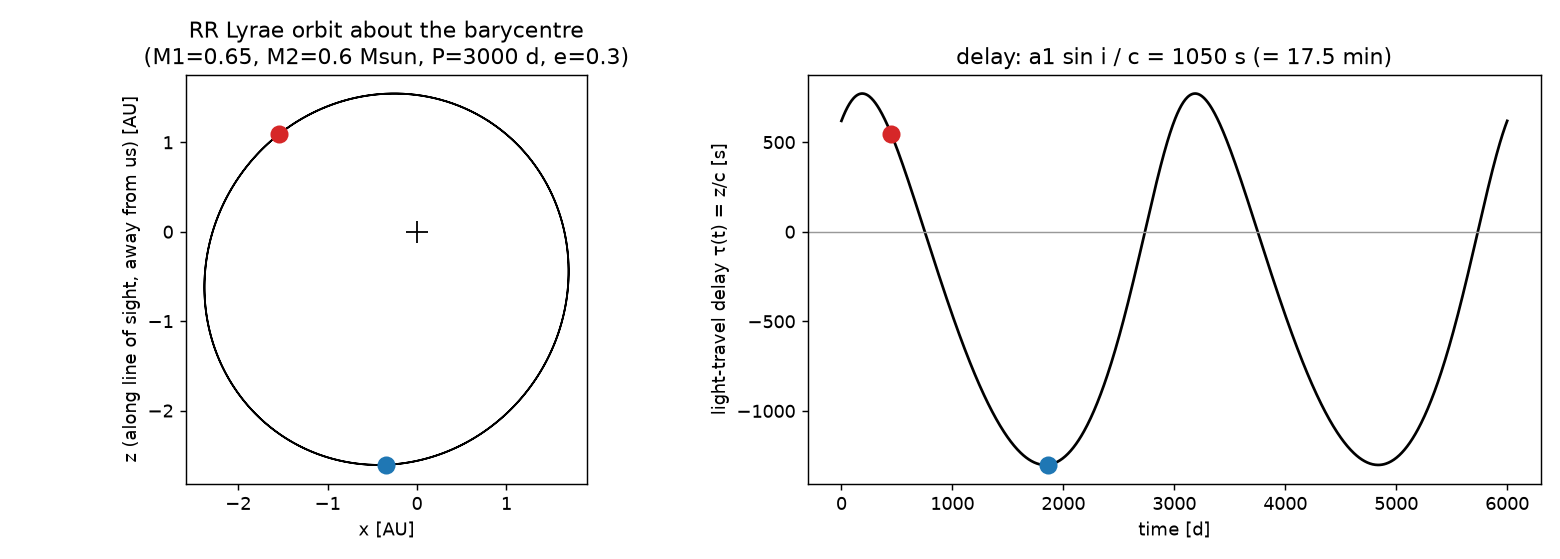
\includegraphics[width=\textwidth]{mock_orbit_delay.png}
\caption{Left: the RR Lyrae's orbit about the barycentre ($+$), with the observer below. Right: the resulting delay
$\tau(t)=z/c$ (\cref{eq:ltte}); the non-sinusoidal shape comes from $e=0.3$. Coloured dots mark the same two epochs
in both panels: far side (red, late) and near side (blue, early).}
\label{fig:orbit}
\end{figure}

\begin{figure}[h]
\centering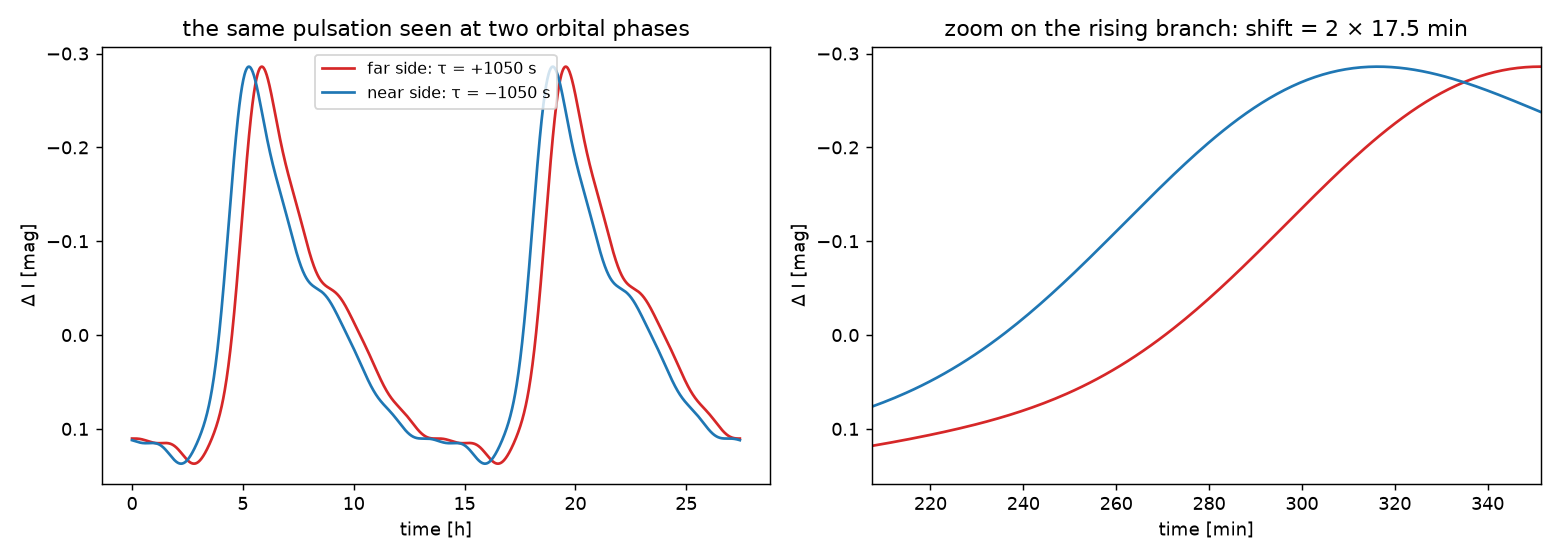
\includegraphics[width=\textwidth]{mock_lightcurve.png}
\caption{The same pulsation observed at the two orbital phases of \cref{fig:orbit}: the light curve is not changed in
shape or amplitude, only shifted in time. Right: zoom on the rising branch, where the shift ($2\times17.5$\,min) is
most easily measured.}
\label{fig:lc}
\end{figure}

\begin{figure}[h]
\centering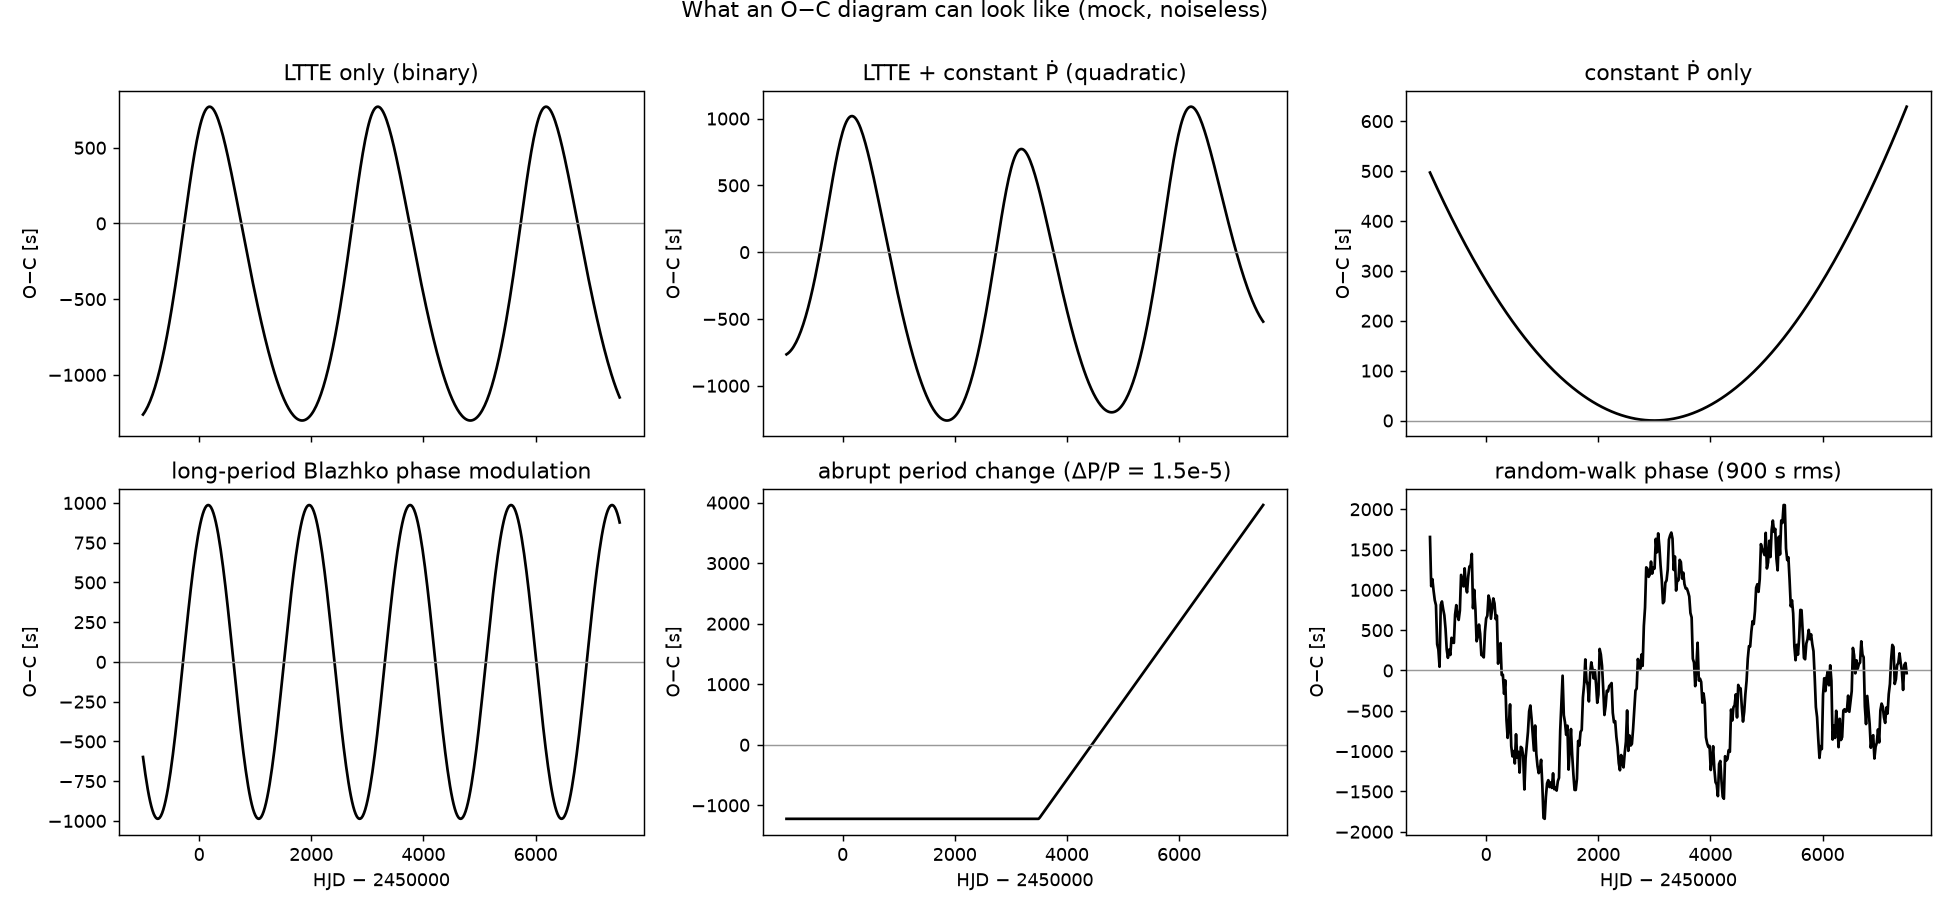
\includegraphics[width=\textwidth]{mock_oc_zoo.png}
\caption{Noiseless mock \OC\ diagrams over the 1992--2016 baseline. Top: binary (LTTE), binary plus constant
\Pdot, constant \Pdot\ only. Bottom: the intrinsic nuisances --- long-period Blazhko phase modulation (periodic, like
an orbit, but accompanied by amplitude changes), an abrupt period change (a broken line), and random-walk phase
wander. Over one or two cycles all three can resemble an orbit.}
\label{fig:zoo}
\end{figure}

\begin{figure}[h]
\centering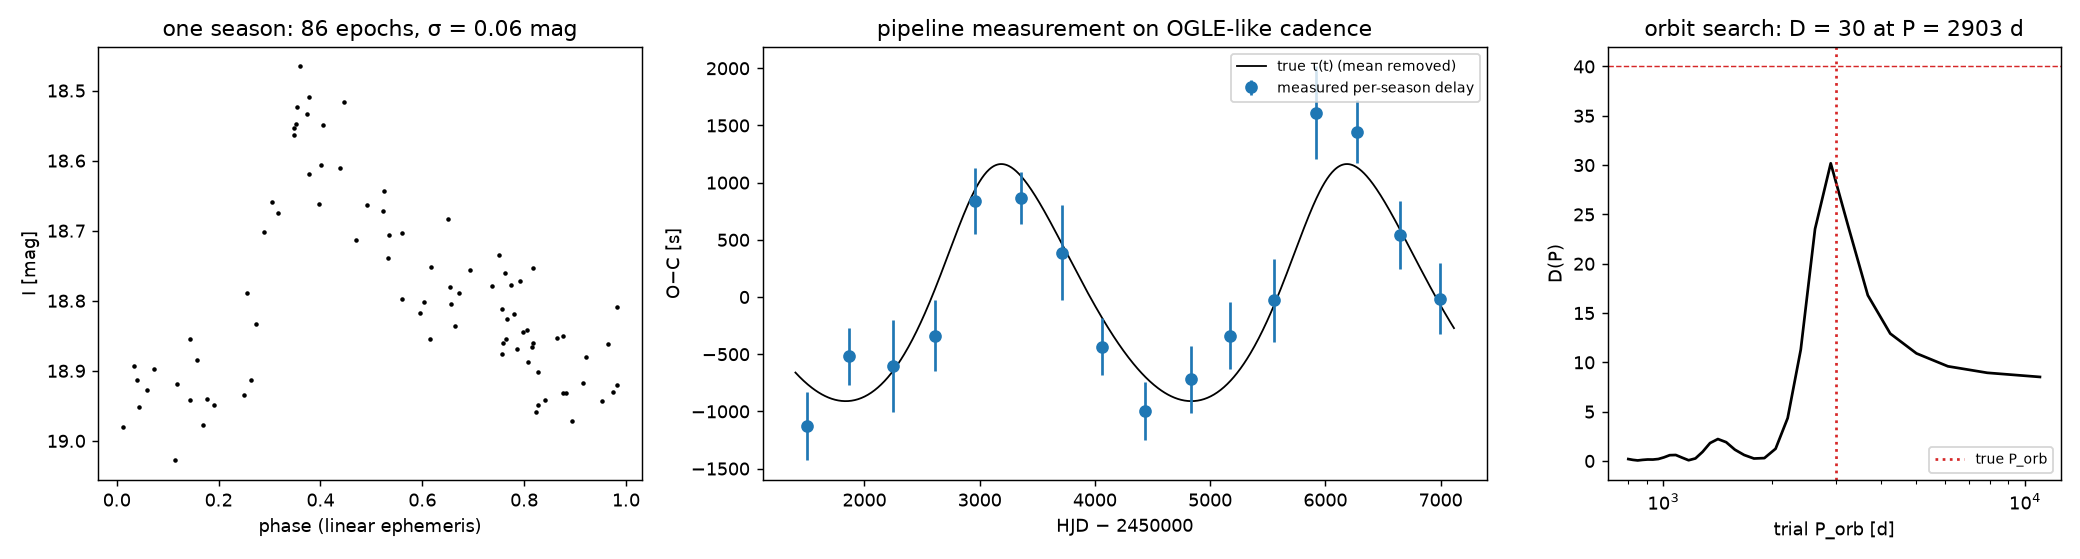
\includegraphics[width=\textwidth]{mock_measurement.png}
\caption{The pipeline on a mock star with an OGLE-III+IV-like cadence (16 seasons, 40--110 epochs each,
$\sigma=0.06$\,mag). Left: one season folded on the linear ephemeris. Middle: measured season delays (median error
297\,s) against the true delay. Right: the orbit search $D(P_{\rm orb})$ (\cref{eq:D}) recovers $P=2903$\,d (true
3000\,d) with $D=30$ --- a 1050-s signal is a firm but not overwhelming detection at LMC photometric precision.}
\label{fig:meas}
\end{figure}

\begin{figure}[h]
\centering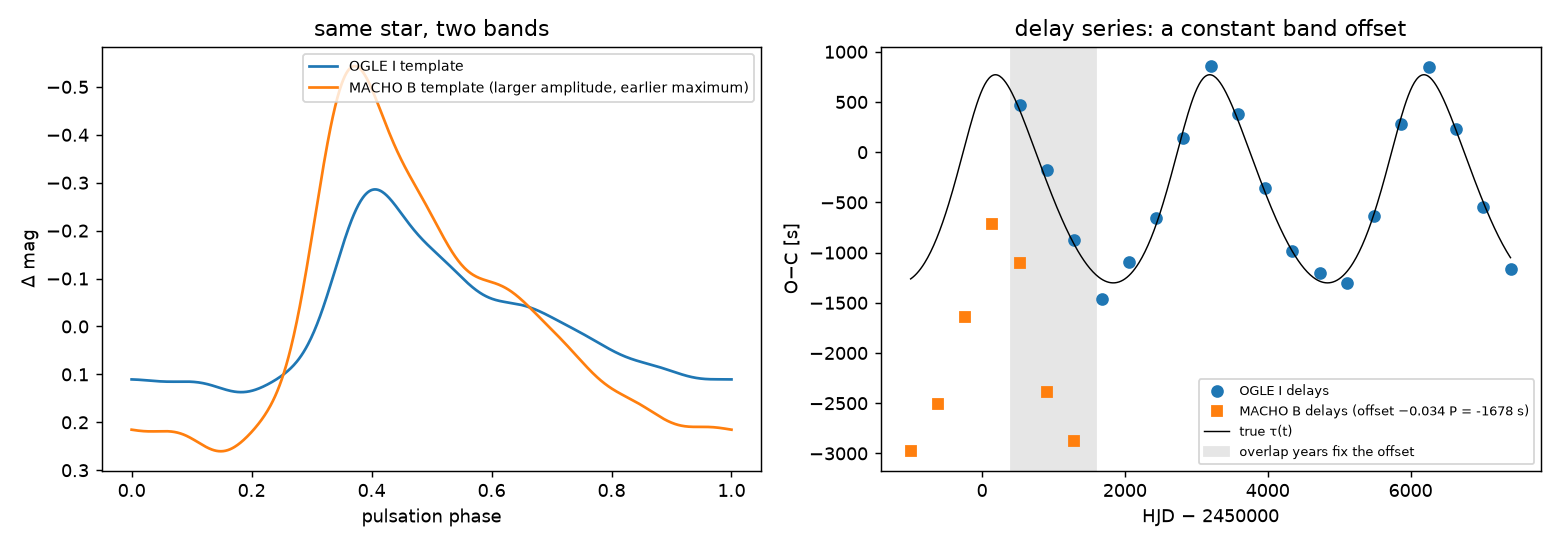
\includegraphics[width=\textwidth]{mock_two_bands.png}
\caption{Two surveys in two bands. Left: MACHO $B$ and OGLE $I$ templates of the same star differ in amplitude and
the maximum occurs 0.034 cycles earlier in $B$ (the measured mean lag, \cref{sec:tie}). Right: hence the MACHO delay
series is offset by a constant from the OGLE series; the years observed by both surveys (grey) fix the offset.}
\label{fig:bands}
\end{figure}

%==============================================================================
\section{The pipeline}\label{sec:pipeline}

\subsection{Data}
\begin{itemize}[leftmargin=*]
\item \textbf{OGLE-IV} LMC RR Lyrae collection \citep{Soszynski2016}: 41{,}471 stars; $I$-band light curves for 41{,}209,
epochs HJD$'$ = 5260--8924, where HJD$'$ = HJD $-$ 2450000 (public data mostly end at 7507, i.e.\ 2016).
\url{https://www.astrouw.edu.pl/ogle/ogle4/OCVS/lmc/rrlyr/}
\item \textbf{OGLE-III} \citep{Soszynski2009}: 24{,}906 light curves, HJD$'=2166$--$4540$ (2001--2008); the 2024
re-issue of the files includes \textbf{OGLE-II} epochs (from HJD$'=447$, 1997) for 7{,}784 stars.
Same star numbering as OGLE-IV (24{,}818 matches, median separation $0.05''$).
\url{https://www.astrouw.edu.pl/ogle/ogle3/OIII-CVS/lmc/rrlyr/}
\item \textbf{MACHO} $B$ and $R$ photometry (1992--1999) via the NCI TAP service
(\url{https://machotap.asvo.nci.org.au/ncitap/tap}), queried per tile for the RR Lyrae only (MACHO IDs from the
OGLE-III cross-identification): 8{,}406 of 8{,}557 requested stars returned. We use MACHO $B$.
\item \textbf{Sample for this note:} 17{,}492 RRab with OGLE-III and OGLE-IV light curves; 6{,}614 with usable MACHO data;
2{,}378 of these also have OGLE-II (overlap years 1997--1999).
\end{itemize}

\subsection{Time system}
OGLE times are HJD (UTC). MACHO \texttt{dateobs} is MJD and is converted to HJD for each star (observer at Mount
Stromlo); towards the LMC, near the south ecliptic pole, the heliocentric correction is only $\pm40$\,s
(tested). Whether MACHO times refer to the start or middle of the exposure is not documented; the band-lag test in
\cref{sec:tie} limits any residual MACHO--OGLE clock offset to $\approx\pm50$\,s.

\subsection{Seasons}
A season is one observing year, with the boundary at HJD$'$ mod 365.25 $=245$ (the middle of the OGLE seasonal gap).
MACHO observed the LMC nearly year-round, so gap-based seasons would merge years. Seasons with fewer than 15 epochs are dropped.

\subsection{Timing fit per star and band}
\cref{eq:lc} with $K=8$, separate zero points per survey segment, per-season $(\tau_j,\delta m_j,\alpha_j)$,
$4\sigma$ clipping, template$\leftrightarrow$delay iterations until the mask is stable and $\max|\Delta\tau|<10^{-7}$\,d,
the fundamental-phase gauge, and errors from \cref{eq:fisher} scaled by $\sqrt{\max(\chi^2_\nu,1)}$. Delays are
defined modulo $P$ and unwrapped between consecutive seasons.
\emph{Measured precision} (1000 random OGLE-III+IV RRab): median season error 253\,s (10--90\%: 121--510\,s), strongly
amplitude-dependent (476\,s for $A_I<0.4$, 113\,s for $A_I>0.8$); MACHO $B$ per year: median 135\,s.

\subsection{Tying MACHO to OGLE}\label{sec:tie}
Band-dependent template shapes leave a constant offset $\Delta$ between the MACHO $B$ and OGLE $I$ delay series
(\cref{fig:bands}). On 781 stars observed by both in 1997--1999: $\Delta/P=-0.034$ cycles (robust scatter 0.008), with
a $\sim300$-s star-to-star scatter. The same behaviour (lag $-0.035$ cycles, similar period dependence and scatter) is
found between OGLE's own $V$ and $I$, which share one time system: the offset is a physical band lag, not a MACHO clock
error. In the \OC\ search $\Delta$ is a free parameter per star (an indicator column); for stars with OGLE-II it is fixed
by the overlap years.

\subsection{Common-mode timing correction}
Stacking all stars' \OC\ residuals by year reveals a common MACHO pattern ($-113$ to $+40$\,s) and a smaller OGLE drift
($+10$ to $+24$\,s in 2006--2008). A null test (white-noise delays at the real epochs, same stacking) is consistent
with zero, so these are real timing systematics; the per-(survey, year) median is subtracted from every star (median
correction 12\,s rms per star; the candidate list is unchanged by it).

\subsection{Orbit search and the annual-sampling limit}\label{sec:nyquist}
$D$ (\cref{eq:D}) is maximized over trial periods uniform in frequency, from 800\,d to twice the baseline. Season
delays sample the \OC\ about once per year, so orbital periods below the Nyquist limit of 2\,yr are aliased: in an
earlier version the grid started at 300\,d and a 3000-d orbit could be assigned its alias at
$1/(1/365.25-1/3000)=416$\,d. \textbf{All statistics based on the earlier grid are being recomputed.}
Orbits shorter than 2\,yr would require within-season timing and are outside the present search.

\subsection{Nuisances and discriminators}\label{sec:nuis}
Simulated on each star's real cadence and errors from its own fitted templates (\texttt{src/rrlbin/simulate.py};
one delay realization shared by MACHO and OGLE): constant \Pdot; Blazhko (coherent phase and amplitude modulation,
$P_B=20$--3000\,d); abrupt period changes ($|\Delta P/P|$ from $10^{-6}$ to $2\times10^{-4}$); random-walk phase (50--15{,}000\,s rms);
LTTE (log-uniform $P_{\rm orb}=300$--$10^4$\,d, $M_2=0.05$--$1.5\,\Msun$, isotropic, half eccentric). Discriminators:
\begin{itemize}[leftmargin=*]
\item amplitude constancy $\chi^2_\nu(\alpha_j)<2$ (Blazhko veto; LTTE does not change amplitude);
\item at least 1.5 orbital cycles within the baseline;
\item a physical ceiling: $A$ below $a_1/c$ for $M_2=2\,\Msun$ at the fitted period (costs 4.5\% of true LTTE; applied
identically to simulations);
\item for stars with OGLE-II: a predictive test (fit from 1997 on, predict the held-out 1992--1996 MACHO delays).
\end{itemize}
Real stars have a heavier tail of timing noise than the nuisances first simulated (jitter 90th/97th percentiles
1.6/3.8\,ks), which motivated the large random-walk and large-jump classes.

\subsection{Code and tests}
Package \texttt{rrlbin} (\texttt{io}, \texttt{timing}, \texttt{ltte}, \texttt{simulate}, \texttt{mixture}); 20 unit tests
(\texttt{pytest}): Fourier derivatives, exact recovery of noiseless delays ($<0.01$\,s), gauge invariance, pull
distributions of noisy delays, Kepler solver and eccentric delay amplitude, LTTE amplitudes of \cref{tab:amp}, mass
function, O$-$C search recovery and null calibration, the annual-Nyquist grid, predictive score, MJD$\to$HJD. Long
runs use a chunked, resumable runner. Full log: \texttt{JOURNAL.md}.

%==============================================================================
\section{Status (to be updated after the re-run)}\label{sec:status}
Before the period-grid fix, the candidate selection ($D>40$, amplitude veto, $A/\sigma>3$, $\ge1.5$ cycles, ceiling)
retained 67 stars (60 with MACHO), several with smooth two-cycle \OC\ curves on 12--14-yr periods
(\cref{fig:cand}). The population mixture fit of the binary fraction was found to be only weakly identified (it
depends on the assumed nuisance shapes by a factor $\gtrsim2$), and a conservative completeness-corrected upper limit
was $f<2.8\%$ (95\%) for $M_2=0.4$--$1.5\,\Msun$, $P_{\rm orb}=1$--$10$\,kd. These numbers will change with the corrected
grid and are \textbf{preliminary}.

\begin{figure}[h]
\centering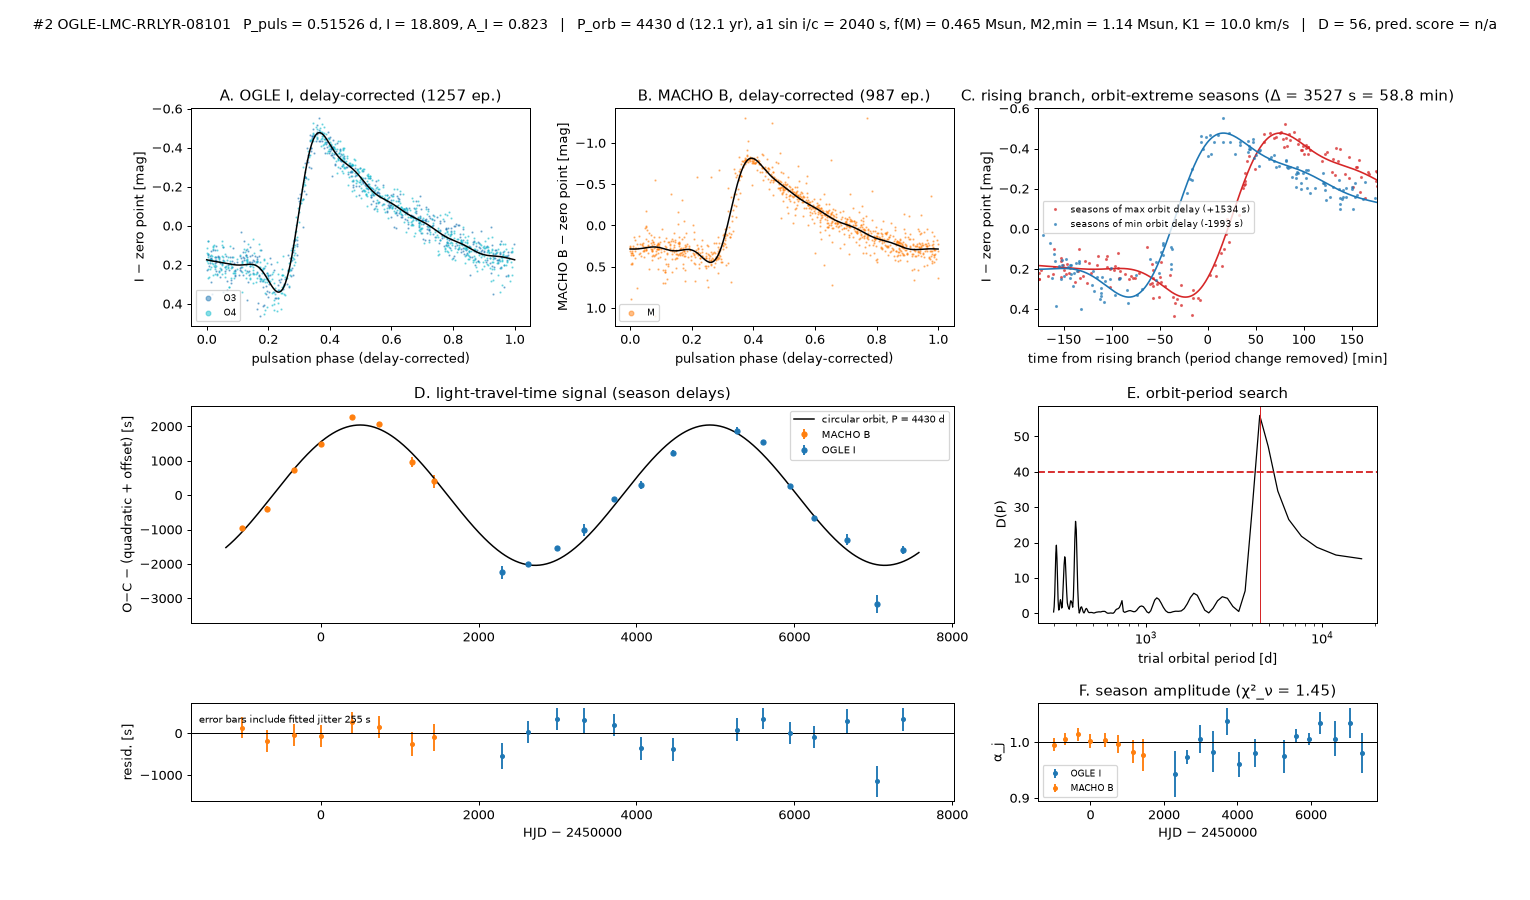
\includegraphics[width=\textwidth]{02_OGLE-LMC-RRLYR-08101.png}
\caption{Example candidate sheet (pre-fix grid; this star's period, 4430\,d, is well above the Nyquist limit and not
affected). A, B: delay-corrected folds (OGLE $I$, MACHO $B$) with templates. C: raw OGLE points on the rising branch in
the seasons of maximum and minimum orbital delay, with the period change removed --- the whole waveform is shifted
by 59\,min. D: \OC\ with the circular-orbit fit and residuals. E: $D(P_{\rm orb})$. F: season amplitudes.}
\label{fig:cand}
\end{figure}

%==============================================================================
\begin{thebibliography}{99}\small
\bibitem[Irwin(1952)]{Irwin1952} Irwin J.\,B., 1952, ApJ, 116, 211, ``The determination of a light-time orbit''.
\url{https://ui.adsabs.harvard.edu/abs/1952ApJ...116..211I}
\bibitem[Soszy\'nski et al.(2009)]{Soszynski2009} Soszy\'nski I., et al., 2009, AcA, 59, 1 (OGLE-III LMC RR Lyrae).
\url{https://arxiv.org/abs/0903.2482}
\bibitem[Soszy\'nski et al.(2016)]{Soszynski2016} Soszy\'nski I., et al., 2016, AcA, 66, 131 (OGLE-IV Magellanic RR Lyrae).
\url{https://arxiv.org/abs/1606.02727}
\bibitem[Hajdu et al.(2015)]{Hajdu2015} Hajdu G., et al., 2015, MNRAS, 449, L113. \url{https://doi.org/10.1093/mnrasl/slv024}
\bibitem[Hajdu et al.(2021)]{Hajdu2021} Hajdu G., et al., 2021, ApJ, 915, 50 (87 bulge LTTE candidates).
\url{https://doi.org/10.3847/1538-4357/abff4b}
\bibitem[Prudil et al.(2019)]{Prudil2019} Prudil Z., et al., 2019, MNRAS, 487, L1. \url{https://doi.org/10.1093/mnrasl/slz069}
\bibitem[Li\v{s}ka et al.(2016)]{Liska2016} Li\v{s}ka J., et al., 2016, A\&A, 589, A94 (TU UMa).
\url{https://doi.org/10.1051/0004-6361/201525870}
\bibitem[Bobrick et al.(2024)]{Bobrick2024} Bobrick A., et al., 2024, MNRAS, 527, 12196 (RR Lyrae from binary evolution).
\url{https://doi.org/10.1093/mnras/stad3996}
\bibitem[Cusano et al.(2021)]{Cusano2021} Cusano F., et al., 2021, MNRAS, 504, 1 (VMC LMC RR Lyrae; blending).
\url{https://doi.org/10.1093/mnras/stab901}
\end{thebibliography}

\end{document}
